\documentclass[uplatex]{jsarticle}
\usepackage{amsmath,amssymb}
\usepackage{float}
\usepackage[scaled]{helvet}
\usepackage{amsthm}
\usepackage{color}
\usepackage[dvipdfmx]{graphicx}
\usepackage{enumitem}

% 定理環境
\theoremstyle{definition}
\newtheorem{df}{定義}[section]
\newtheorem{theo}[df]{定理}
\newtheorem{prop}[df]{命題}
\newtheorem{lemm}[df]{補題}
\newtheorem{cor}[df]{系}
\newtheorem{ex}[df]{例}
\newtheorem{fact}[df]{事実}
\newtheorem{nex}[df]{反例}

\newcommand{\indep}{\mathop{\,\perp\!\!\!\!\!\perp\,}}
\newcommand{\notindep}{\mathop{\,\perp\!\!\!\!\!/\!\!\!\!\!\perp\,}}

%
% \qed を自動で入れない proof 環境を再定義
%
\makeatletter
\renewenvironment{proof}[1][\proofname]{\par
  \normalfont
  \topsep6\p@\@plus6\p@ \trivlist
  \item[\hskip\labelsep{\bfseries #1}\@addpunct{\bfseries.}]\ignorespaces
}{%
  \endtrivlist
}
\renewcommand{\proofname}{証明}
\newcommand{\relmiddle}[1]{\mathrel{}\middle#1\mathrel{}}
\makeatother


\title{マーケティング・リサーチにおける \\ 統計的因果探索を用いた因果仮説構築に関する研究}
\author{データサイエンス研究科, 株式会社マクロミル \\ 小西 伶児}
\date{\today}


\begin{document}
%% Front Matter
%\frontmatter{}
%
%!TEX root = ../thesis.tex

\maketitle
%
\section*{概要}
\thispagestyle{empty}
%
本研究では,

%
\tableofcontents
%
%\listoffigures
%
%\listoftables
%

%
%% Main Matter
%
\section{序論}
\label{part:introduction}

あああ
%
%!TEX root = ../thesis.tex

\subsection{研究背景}

企業は自社の商品やサービスを顧客に提供するために、様々なマーケティング活動を行っている。
近年では消費者の嗜好が多様化したり、新型コロナウイルス感染症が流行したりするなど、
企業活動を取り囲む環境が日々大きく変化しており、
企業はその環境変化に適応する必要がある。
それ故、商品・サービスの開発や消費者とのコミュニケーションなどのマーケティング活動を
適切に実行するためには、消費者の行動について深く理解することがより一層重要となっている。

アメリカ・マーケティング協会(AMA)によると、
マーケティングの定義は「顧客、クライアント、パートナー、社会のための
価値の創造、伝達、提供、交換という全体の活動」であり、
マーケティング・リサーチは「消費者、顧客、公衆とマーケターが情報を介してつながる機能」である
と定義している\cite{AMA_marketing}。
また、その具体的な業務として、
「必要な情報を特定し、情報収集のための方法を設計し、データ収集プロセスを管理・実施し、
結果を分析し、分析結果と結果から得られる示唆伝えること」としている。
つまり、上記の定義を合わせて考えると、マーケティング・リサーチの目的は
「マーケティング課題の発見や施策の実行に必要なデータを適切に収集し、
得られたデータを分析することで、企業のマーケティング活動を支援すること」と理解することができる。

企業のマーケティング活動は、主に以下の4つのフェーズに分類することが可能で、
商品・サービスのカテゴリにも依存するが、約1〜数年程度の期間で繰り返されることが一般的である。
この繰り返しのことをマーケティング・サイクルと呼ぶ。
\begin{itemize}
  \item 市場機会の発見
  \item コンセプト開発
  \item コミュニケーション内容・販売施策の策定
  \item 施策後の効果検証
\end{itemize}
マーケティング・リサーチは、各フェーズにおけるマーケティング担当者の関心事に対して、
適切な示唆を与えることが求められている。
%コトラーは「誰に対してどのような価値を提供するのか」というマーケティングの目的を達成するために、
%消費者を細分化(セグメンテーション)し、
%その中でどのセグメントを優先的に自社の顧客とするのか(ターゲティング)を明確にし、
%他商品との関係性を設定すること(ポジショニング)が必要不可欠だと指摘している\cite{Kotler1999-im}。
「市場機会の発見」では、
「市場にある商品で満たされていないニーズは何か?」や
「この商品を購入している人はどのような特徴があるのか?」といったことが
マーケティング担当者の関心事となり、
未充足ニーズの探索や、消費者セグメントの整理などがリサーチの役割となる。
次に「コンセプト開発」では、
「どのような価値を提供すると売れるのか?」や
「ターゲットとなる消費者の規模はどのくらいか?」といったことが関心事となり、
コンセプトの受容性確認や、消費者セグメントの規模感把握などがリサーチに求められる。
また「コミュニケーション内容・販売施策の策定」では、
「商品の特長をどのように伝えると購買に結びつくのか?」や
「商品パッケージや価格はどのようにすればよいか?」といったことが主な関心事となり、
広告内容の精査や、商品の改善点抽出などが行われる。
最後に「施策後の効果検証」においては、
市場浸透度の確認や、広告などの投資に対する売上の費用対効果などが行われる。
各フェーズでのマーケティング担当者の関心事を俯瞰すると、
多くは「マーケティング活動と消費者行動の因果関係」にあると言える。

「マーケティング」の他に「ブランディング」も類似の意味を持つ言葉として頻繁に用いられるが、
それぞれの言葉の意味には異なる部分が存在する。
音部(2019)\cite{2019-eb}によると、マーケティングは属性の順位を変換して市場を創造することを目指し、
結果的にニーズを作り出すことにつながっており、
ブランディングはブランドの意味の確立を目指し、結果的にベネフィットを作り出すことにつながっている。
つまり、「マーケティング」は消費者行動の因果構造そのものを変化させることによって、
自社の商品が有利に購買されるような状況を作り出す活動であることに対し、
「ブランディング」は現在の消費者行動の因果構造はそのままに、
自社の商品に対する消費者の認識を変化させることによって、
他社の商品ではなく自社の商品を購買するように行動を変化させる活動であると
捉えることができる。

このように、企業は自社の商品やサービスを顧客に効率的に提供するために、
マーケティング・リサーチを通じて消費者に関する情報を収集・分析し、
消費者行動の因果関係について仮説を立てたり解釈を行ったりしている。
そのため、マーケティング・リサーチにおいて、消費者行動の因果関係に関する情報を得る手段は、
非常に重要な役割を担っている。

%
%!TEX root = ../thesis.tex

\subsection{既存手法・研究}

因果関係に関する考察は、科学の基本的な問いとして因果推論という文脈で研究されてきた。
近年では計算機科学や統計科学の発展により、経済学やマーケティングの分野でも注目されている\cite{Varian2016-se}。
因果推論は大まかには、
(i)因果構造の同定、と
(ii)因果構造を既知としたその因果関係の大きさの推定、
という2つの問題に分類できる。
(i)因果構造の同定 は、非常に困難な問題であるとされているが、
いくつかの仮定の上で識別可能なモデルが提案されている。
(ii)因果構造を既知としたその因果関係の大きさの推定 は、
ランダム化比較試験を中心とした実験研究と、
特に実験を行わない観察研究の双方において統計科学の文脈で研究されている。

本節では、マーケティング・リサーチにおいて消費者行動の因果関係に関する情報を得る方法として
従来より広く用いられてきた一般的な既存手法について述べた後、
統計的因果探索と呼ばれる因果構造の同定に関する近年の研究について俯瞰する。

\subsubsection{マーケティング・リサーチにおける既存手法}

マーケティング・リサーチは大きく定性調査と定量調査に分類され、
それぞれにおいて消費者行動の因果関係に関する情報の分析を行う。

定性調査は一般的に、消費者の内部にある意見や態度を理解することで、
マーケティング課題の詳細な定義、仮説の設定、定量調査における調査項目の優先順位の決定、
消費者独自の考え方や表現の理解、企業のマーケティング担当者の不足している知識の吸収、
定量調査における最重要な項目に関する示唆を得るなどの目的で実施される\cite{2018-ci}。
主に深層面接法(デプス・インタビュー)や集団面接法(グループ・インタビュー)といった、
インタビュアーが回答者との対話を通じて質問をし回答を得る方法が一般的である。
そのため、調査対象者が日常生活であまり気に留めていないことや、
誰かに問いかけられて初めて気づくことなどを収集することができ\cite{2018-ci}、
マーケティング担当者の周辺知識では想定しきれなかった因果関係を発見できる可能性がある。
一方で、定性調査は定量調査と比べて一般的に時間や費用が多くかかることや、
定量的な評価ができず、得られた意見や行動の一般性・代表性に関する議論ができないことなどの
デメリットがある。

定量調査では、主にアンケート調査に代表される意識データや、
POSデータ、ID付きPOSデータ、位置情報などの行動データが用いられる。
これらのデータの分析手法は非常に多岐に渡るが、
消費者行動の因果関係を評価する手法としては、
一般化線形モデル(generalized linear model, GLM)や
構造方程式モデル(structural equation model, SEM)を用いることが多い\cite{2015-pb}\cite{2009-qw}。
GLMでは、目的変数と説明変数の関係を定式化し、
各係数を目的変数に対する説明変数の因果関係の大きさとして解釈を行うことが慣例となっている。
しかし、宮川(2004)\cite{2004-qj}で述べられている通り、
GLMは説明変数を与えたときの目的変数の条件付き確率分布に関するモデルである。
つまり、GLMによる分析の目的は、説明変数を観測したときの目的変数の予測であり、
説明変数に外的操作を行ったときの目的変数の因果効果の定量化ではない。
そのため、推定されたパラメータに対して因果的な解釈を行うことは誤りとなる可能性がある。
一方で、SEMはデータの生成過程を記述した統計的因果モデルであり、
その係数は単なる相関関係の尺度ではなく、因果的な解釈を行うことができる\cite{2004-qj}。
ただし、SEMは分析者の事前知識を積極的に利用することで因果構造の仮説を有向グラフで表現した上で、
その構造に対してモデリングを行う手法である。
つまり、SEMは上述の(ii)因果構造を既知としたその因果関係の大きさの推定を行う手法であると言える。
そのため、因果構造の仮説構築は分析者側の事前知識の質や量に依存し、
妥当だと思われるモデルを得るまでに長い時間を要したりしているという現状がある。
また、近年の社会の発展により消費者の行動は複雑化しているため、
因果構造に関する仮説を構築することが難しい場合も少なくない。


\subsubsection{統計的因果探索}

統計的因果探索とは、因果構造が未知である際に、
どのような条件の下で観測データから因果構造が復元することが可能であるかを明らかにし、
観測データがその条件を満たしているという仮定の下で、
因果構造を推定する手法を研究する学問分野である。
マーケティング・サイエンスを含む多くの実質科学の分野では、
様々な現象の因果関係に関する分析が行われているが、
因果仮説を1つに絞りきれない場合や、
その分野の背景理論が不足しており因果仮説を立てられない場合がある。
そのような場合に統計的因果探索が活用できることが期待されている\cite{2017-zx}。

統計的因果探索の分野において、因果関係を復元するための手がかりの1つは、
因果構造の特徴を示す統計的関連性のパターンである\cite{Pearl2009-oh}。
例えば、2つの公平なサイコロを振った時に得られる結果を$A, B$とし、
2つのサイコロの出た目の合計を$C$とする。
この時、$A$と$C$、$B$と$C$は従属しているが、
$A$と$B$は独立であるという3つの統計的関連性が得られる。
しかし、$C=6$という状況の下では$A$と$B$は従属する。
このことを直感的にグラフに表現すると、
$A \rightarrow C \leftarrow B$となる。
実際、$C=A+B$であるため、$A$と$B$は$C$の原因である。
つまり、統計的関連性(条件付き独立性)を用いることで、
因果構造を復元することが可能な場合があると言える。
しかし、因果構造が異なる場合でも
観測データから同じ条件付き独立関係が得られる場合も多い。
例えば、
$X \rightarrow Y \rightarrow Z$、
$X \leftarrow Y \rightarrow Z$、
$X \leftarrow Y \leftarrow Z$という3つの異なる因果構造から生成された観測データは、
全て「$Y$で条件付けると$X$と$Z$が独立である$(X \indep Z | Y)$」という
条件付き独立関係のみが得られる。
つまり、条件付き独立性を用いるだけでは3つの因果構造を識別することができない。
この条件付き独立性から区別できない因果構造のことをマルコフ同値類(観察的同値類)と言う\cite{Pearl2009-oh}。
そのため、一般に観察データから因果構造を一意に復元することは非常に困難であると言える。

そこで、データ生成過程に関する様々な仮定をおくことで、
因果構造を一意に復元できる識別可能な因果モデルが複数示されている。
観測変数が全て連続である場合は、
変数間の関係性を表す関数が線形であり、外生変数の分布が非正規分布であることを仮定したLiNGAM\cite{Shimizu2006-yu}、
関数形が非線形であるAdditive Noise Model(ANM)\cite{Hoyer2008-oo}、
関数形が線形であり誤差変数の分散が全て等しい、または全て既知である正規線形構造方程式モデル\cite{Peters2013-eb}
などが挙げられる。

次に、観測変数が全て離散である場合は、
各変数の条件付き分布がポアソン分布に従うことを仮定した
Poisson DAGモデル\cite{Park2015-tj}、
関数形にブール関数などの離散変数を扱う関数を仮定したANM\cite{Peters2011-ew}
などが挙げられる。

最後に、連続変数と離散変数が混在する場合の研究について述べる。
各変数の条件付き分布の分散が期待値の2次式で表現できるという
2次分散関数(QVF)DAGモデル\cite{Park2017-hw}がある。
これはPoisson DAGモデル\cite{Park2015-tj}を拡張することによって
識別可能性が示されている。
分散が期待値の2次式で表現できる分布には、
ポアソン分布や二項分布、幾何分布などの離散確率分布だけでなく、
指数分布やガンマ分布などの連続確率分布も含まれており、
連続変数と離散変数が混在する場合でも適用できる手法である。
ただし、各変数の条件付き分布については事前に仮定をおく必要がある。
また、離散変数が2値(0,1)であることを仮定したモデルには、
混合因果モデル\cite{Wenjuan2018-nm}やハイブリッド因果モデル\cite{Li2018-aw}
などがある。
ただし、これらのモデルは一般的な$p$変数における識別可能性は示されていない。

%
%!TEX root = ../thesis.tex

\subsection{研究目的}

あああ
aaa

%
%!TEX root = ../thesis.tex

\subsection{本論文の構成}

まず2章では、
本研究の基礎となる統計的因果探索の従来研究として、
連続変数を扱うANMと
離散変数を扱うQVF DAGモデルについて述べる。
3章では、Park and Park(2019)\cite{Park2019-qy}のアイデアを用いて
QVF DAGモデルの識別可能性を証明する。
4章では、ANMとQVF DAGモデルを用いることによって、
連続変数と離散変数が混在する構造的因果モデルを提案し、その識別可能性を証明する。
5章では、4章で提案したモデルを推定する手法について述べる。
6章では、数値実験によって、予め設定した因果構造に基づいてデータを発生させ、
その因果構造の推定を行う。
数値実験の結果、従来手法と比較して提案手法が有効であることを示す。
最後に7章では、本論文のまとめと今後の課題について述べる。


%
%!TEX root = ../thesis.tex

\section{既存モデル}
\label{part:model}

本章ではまず、本論文で用いる数学記号を導入し、
非巡回有向グラフ(Directed Acyclic Graph, DAG)モデルとその識別可能性を定義する。
その後、本論文の提案モデルを構成する2つの既存モデルについて概説する。
既存モデルの1つ目は、連続変数を扱うDAGモデルとして広く用いられている
Additive Noise Model
\cite{Shimizu2006-yu}
\cite{Hoyer2008-oo}
\cite{Peters2013-eb}
\cite{Peters2014-ro}
\cite{Park2020-ey}
である。
2つ目は、主に離散変数を扱うDAGモデルで、
Park and Raskutti(2017)\cite{Park2017-hw}によって提案された
2次分散関数(Quadratic Variance Function, QVF)DAGモデルである。
%QVF-DAGモデルの識別可能性は、Park and Raskutti(2017)\cite{Park2017-hw}によって
%過分散スコアを用いて証明されたが、
%本論文ではPark and Park(2019)\cite{Park2019-qy}が提案した
%モーメント比スコアを拡張することで、識別可能条件の緩和を行う。



%
%!TEX root = ../thesis.tex

\subsection{数学的準備}

グラフは頂点(node)の集合$V=\{1,2,\dots,p\}$と、
頂点同士をつなぐ辺(edge)の集合$E\subset V \times V$ によって、
$G=(V,E)$と表現される。
グラフの辺は有向辺(矢線)と無向辺(双方向矢線)に分けることができ、
2つの頂点$j,k\in V$において、
$(j,k)\in E$かつ$(k,j)\notin E$のとき、$j$から$k$への矢線があるという。
これを$j \rightarrow k$と表現することもある。
一方で、$(j,k)\in E$かつ$(k,j)\in E$のとき、$j$と$k$の間に双方向矢線があるという。
すべての辺が有向辺であるグラフを有向グラフ(directed graph)という。
本論文では、特に断りのない限り、頂点$j$から$k$への矢線がある場合、
$j$が$k$の原因であるといった因果関係があることを表すとする。
つまり、本論文で扱うグラフにおける矢線の有無は因果関係の有無を表しており、
矢線の始点が原因で、矢線の終点が結果である。
このような定性的な因果関係を表すグラフを因果グラフ(causal graph)という。
また、グラフ$G$からすべての矢印を取り除くことによって得られるグラフを
$G$のスケルトンという。

頂点の系列$\alpha_1, \alpha_2, \dots, \alpha_{n+1}$について、
すべての$i=1,2,\dots, n$で、
$\alpha_i \rightarrow \alpha_{i+1}$、または$\alpha_{i+1} \rightarrow \alpha_i$となる矢線がある時、
長さ$n$の道(path)という。
特に、すべての$i=1,2,\dots, n$で、$\alpha_i \rightarrow \alpha_{i+1}$となる矢線がある時、
長さ$n$の有向道(directed path)という。
また、長さ$n$の有向道で、$\alpha_1 = \alpha_{n+1}$となるものを巡回閉路(cycle)という。
一方で、巡回閉路のない有向グラフは非巡回的(acyclic)であるという。
本論文では、非巡回有向グラフ(Directed Acyclic Graph; DAG)のみを扱う。

頂点$j$から$k$への矢線がある時、$j$を$k$の親(parent)といい、$k$を$j$の子(child)という。
また、$(j,k)\in E$であるすべての頂点$j$からなる集合を$Pa(k)$と表記する。
頂点$j$から$k$への有向道がある時、$j$を$k$の祖先(ancestor)、
$k$を$j$の子孫(descendant)という。
頂点$k$のすべての祖先からなる集合を$An(k)$、すべての子孫からなる集合を$De(k)$と表記する。
また、すべての頂点から$k$と$k$の子孫を除いたものを、$k$の非子孫(non-descendant)といい、
その集合を$Nd(k) \equiv V \backslash (\{k \} \cup De(k))$と表記する。
さらに、因果的順序(causal oredering)について定義する。
因果的順序とは、その順序に従って変数を並び替えると、
すべての矢線$(j,k)\in E)$について、$k$が$j$の原因になることがない順序のことであり、
$\pi =(\pi_1, \dots, \pi_p)$と表記する。
DAGで表現される因果グラフには、このような順序が(一意とは限らないが)存在するという特徴がある。
つまり、因果グラフを同定することは、因果的順序を同定することとスケルトンを同定することという
2つの工程に分解することができる。

有向グラフ$G$における頂点上の標本空間$\mathcal X_V$の確率分布に従う
確率変数の集合$X \equiv (X_j)_{j \in V}$について考える。
ここで、確率変数ベクトル$X$は、同時確率密度関数$f_G(X)=f_G(X_1, X_2, \dots, X_p)$で与えられていると仮定する。
$V$の任意の部分集合$S$について、$X_S \equiv \{X_j:j\in S \subset V \}$と
$\mathcal X_S \equiv \times_{j \in S} \mathcal X_j$を定義する。
ただし、$\mathcal X_j$は$X_j$の確率空間である。
また、任意の頂点$j\in V$について、
確率変数ベクトル$X_S$を与えたときの変数$X_j$の
条件付き確率を$f_j(X_j|X_S)$と表記する。
すると、DAG $G$によるモデルは以下のように因数分解することができる\cite{Pearl2009-oh}。

\begin{equation}
  f_G(X)=f_G(X_1, X_2, \dots, X_p) = \prod_{j=1}^p f_j(X_j | X_{Pa(j)})
  \label{eq:factorization}
\end{equation}

ここで、$f_j(X_j | X_{Pa(j)})$は、$X_j$の
親変数$X_{Pa(j)} \equiv \{ X_k:k\in Pa(j) \subset V \}$を与えた条件付き確率である。

また、本論文では観察データから因果グラフを同定するという問題を扱うため、
因果グラフの識別可能性について定義する。
識別可能性を直感的に説明すると、条件付き確率分布$f_j(X_j|X_{Pa(j)})$に対してある仮定を置くと、
同時確率密度関数$f_G(X)$を与えたDAG $G$の構造を一意に決定付けることができるということである。

識別可能性について詳細に定義するために、すべての$j \in V$に関する
条件付き確率分布$f_j(X_j|X_{Pa(j)})$の集合を$\mathcal P$と表記する。
また、グラフ$G=(V,E)$について、グラフ$G$に関する同時分布のクラスと、
分布$\mathcal P$のクラスを以下で定義する。

\begin{equation}
  \mathcal F(G;\mathcal P) \equiv \{ f_G(X) = \prod_{j \in V} f_j(X_j|X_{Pa(j)}) ;
  \text{where} f_j(X_j|X_{Pa(j)}) \in \mathcal P \quad \forall j \in V \}
\end{equation}

続いて、$p$個の変数からなる非巡回的有向グラフの集合を$\mathcal G_p$と表記する。
そこで、DAG $\mathcal G_p$の空間上の確率分布のクラス$\mathcal P$における
識別可能性を以下のように定義する。

\begin{df}[識別可能性]
  条件付き分布のクラス$\mathcal P$が$\mathcal G_p$において識別可能であるとは、
  $G,G' \in \mathcal G_p$において$G \neq G'$であるならば、
  $f_G = f_{G'}$を満たすような$f_G \in \mathcal F(G; \mathcal P)$と
  $f_G' \in \mathcal F(G'; \mathcal P)$が存在しないことである。
\end{df}

%
%!TEX root = ../thesis.tex

\subsection{Additive Noise Model}

本節では、連続変数データを扱うDAGモデルとして、
広く用いられているAdditive Noise Model(ANM)
\cite{Shimizu2006-yu}
\cite{Hoyer2008-oo}
\cite{Peters2013-eb}
\cite{Peters2014-ro}
\cite{Park2020-ey}
とその識別可能性について概説する。

ANMは、観測変数の同時分布が、
以下の構造方程式と誤差から生成されるDAGモデルである。

\begin{equation}
  X_j = f_j(X_{Pa(j)}) + e_j , \quad e_j \sim (0, \sigma_j^2)
  \label{def:ANM}
\end{equation}

ここで、$(f_j)_{j\in V}$は任意の関数であり、
$(e_j)_{j\in V}$は平均ゼロでそれぞれ異なる分散$(\sigma_j^2)_{j\in V}$に従う
互いに独立な確率変数である。

また、ANMの特殊形として、$(f_j)_{j\in V}$が全て線形な関数で記述されるモデルを、
線形構造方程式モデル(SEM)という。
つまり、観測変数の同時分布が以下の線形方程式で定義されるDAGモデルである。

\begin{equation}
  X_j = \theta_j + \sum_{k \in Pa(j)} \theta_{jk} X_k + e_j, \quad e_j \sim (0, \sigma_j^2)
\end{equation}

ここで、それぞれの係数$\theta_{jk}$は、DAG $G$における頂点$k$から頂点$j$の
直接的な因果効果の大きさを表す。
つまり、頂点$k$が頂点$k$の親であるときは$\theta_{jk} \neq 0$であり、
それ以外のときは$\theta_{jk}=0$である。

これらのDAGモデルは、関数形や誤差変数の分布についていくつかの制約を課すと、
識別可能であることが証明されている。
代表的な識別可能条件について以下に簡単にまとめる。

\begin{itemize}
  \item
  全ての関数$(f_j)_{j \in V}$が非線形である非線形ANM\cite{Hoyer2008-oo}

  \item
  全ての関数$(f_j)_{j \in V}$が線形であり、
  観測変数$(X_j)_{j \in V}$または誤差変数$(e_j)_{j\in V}$のいずれかの確率分布が、
  非ガウス分布に従う線形非ガウス非巡回モデル(LiNGAM)\cite{Shimizu2006-yu}

  \item
  全ての関数$(f_j)_{j \in V}$が線形であり、
  誤差変数$e_j$の分散が全て等しい、または全て既知である線形ANM\cite{Peters2013-eb}
\end{itemize}

%
%!TEX root = ../thesis.tex

\subsection{2次分散関数 (QVF) DAGモデル}

本節では、主に離散変数を扱うDAGモデルとして、
Park and Raskutti(2017)\cite{Park2017-hw}によって提案された
2次分散関数 (QVF) DAGモデルについて概説する。
QVF-DAGモデルは、各頂点の親による条件付き分布$\mathcal P$の分散が、
期待値の2次式で与えられているというモデルであり、
以下のように定義される。

\begin{df}[QVF-DAGモデル\cite{Park2017-hw}]
2次分散関数(Quadratic variance function, QVF)DAGモデルは、
各頂点の親による条件付き確率分布が、
以下で表現される2次分散関数性(quadratic variance function property)を
満たすようなDAGモデルである。

すべての$j \in V$について、以下を満たすような$\beta_{j0}, \beta_{j1} \in \mathbb R$が存在する。
  \begin{equation}
      \mathrm{Var}(X_j|X_{Pa(j)}) = \beta_{j0} E(X_j | X_{Pa(j)}) + \beta_{j1} E(X_j | X_{Pa(j)})^2
      \label{QVF}
  \end{equation}
\end{df}

2次分散関数性を満たす確率分布のクラスには、
ポアソン分布、二項分布、負の二項分布、ガンマ分布などが含まれることが知られている。
これらの確率分布における$\beta_0, \beta_1$を表\ref{table:beta}に示す。

\begin{table}[ht]
  \begin{center}
    \caption{2次分散関数性を満たす確率分布における$\beta_0, \beta_1$の例}
    \begin{tabular}{llcc} \toprule
      確率分布     & $\mathcal{P}$                  & $\beta_0$ & $\beta_1$       \\ \midrule
      ポアソン分布  & $\text{Poisson}(\lambda)$      & 1         & 0               \\
      二項分布     & $\text{Binomial}(N, p)$        & 1         & $-\frac{1}{N}$   \\
      負の二項分布  & $\text{NegativeBinomial}(R,p)$ & 1         & $\frac{1}{R}$    \\
      ガンマ分布   & $\text{Gamma}(\alpha, \beta)$   & 0         & $\frac{1}{\alpha}$ \\ \bottomrule
    \end{tabular}
    \label{table:beta}
  \end{center}
\end{table}

DAGモデルにおいては、各頂点の分布がその頂点の親変数の影響を受けており、
各頂点の条件付き期待値は、任意の単調で微分可能な
リンク関数$g_j \colon \mathcal X_{Pa(j)} \rightarrow \mathbb R^+$によって、
$E(X_j|X_{Pa(j)}) = g_j(X_{Pa(j)})$で表現される。
本論文の後半では、各頂点間の関係について線形性を仮定するため、
QVF-DAGモデルのリンク関数$g_j$がパラメータに関して線形であることを仮定した
QVF構造方程式モデル(structural quation model, SEM)を導入する。

\begin{equation}
  g_j(X_{Pa(j)}) = g_j \left(\theta_j + \sum_{k \in Pa(j)} \theta_{jk}X_k \right)
\end{equation}

ここで、$(\theta_{jk})_{k \in Pa(j)}$は親変数の重み付け係数である。
例えば、ある頂点の条件付き確率分布がポアソン分布の場合、
$g_j(X_{Pa(j)}) = \exp(\theta_j + \sum_{k \in Pa(j)} \theta_{jk}X_k)$
となる。

より一般的には、指数分布族の定義を用いて、以下のように表現することができる。
\begin{equation}
  P(X_j|X_{Pa(j)}) = \exp \left( \theta_{j}X_j  + \sum_{(k,j)\in E} \theta_{jk}X_k X_j -
  B_j(X_j) - A_j \left( \theta_{j} + \sum_{(k,j) \in E} \theta_{jk} X_k \right) \right)
\end{equation}

ここで、$A_j(\cdot)$は対数分配関数(log-partition function)、
$B_j(\cdot)$は指数分布族によって決まる関数、
$\theta_{jk}\in \mathbb R$は頂点$j$に対応するパラメータである。
DAGモデルの因数分解~\eqref{eq:factorization}により、QVF-SEMの同時確率分布は、
以下のように記述することができる。

\begin{equation}
  P(X) = \exp \left( \sum_{j\in V} \theta_{j}X_j + \sum_{(k,j)\in E} \theta_{jk}X_k X_j
  - \sum_{j \in V} B_j(X_j) - \sum_{j \in V} A_j
  \left( \theta_{j} + \sum_{(k,j)\in E} \theta_{jk} X_k \right)\right)
  \label{eq:QVF_factorization}
\end{equation}

このモデルは、関数$A_j(\cdot)$や$B_j(\cdot)$が頂点$j$によって異なることを許容するため、
各条件付き分布がそれぞれ異なる分布に従っているような混合DAGモデルを表現することも可能である。
また、各頂点の分布$\mathcal P$が式~\eqref{QVF}で定義される2次分散関数性を満たす場合、
非線形モデルやノンパラメトリックモデルに拡張することも可能である。


%
%!TEX root = ../thesis.tex

\section{QVF-DAGモデルの識別可能性}
\label{part:newidentifiability}

%
%!TEX root = ../thesis.tex

% \subsection{QVF-DAGモデルの識別可能性}

本章では、前章で導入したQVF-DAGモデル\cite{Park2017-hw}が識別可能であることを証明する。
QVF DAGモデルの識別可能性は
Park and Raskutti(2017)\cite{Park2017-hw}によって
過分散スコア(OverDispersion Score; ODS)を用いて初めて証明された。

過分散とは、ポアソン分布などの分散が期待値に依存する確率分布において、
期待される分散より標本分散の方が大きくなることである。
過分散が生じる原因の1つとして、サンプルの個体差などが挙げられる。
このような個体差などの効果を組み込んだ統計モデルに
一般化線形混合モデル(generalized linear mixed model; GLMM)がある\cite{2012-iq}。

統計的因果探索の文脈において最初に過分散を利用した例は、
Park and Raskutti(2015)\cite{Park2015-tj}のPoisson DAGモデルである。
Park and Raskutti(2015)\cite{Park2015-tj}では
Poisson DAGモデルの各頂点の条件付き分散が過分散であるかどうかを検定することによって
識別可能性を証明している。
Park and Raskutti(2017)\cite{Park2017-hw}では、
Poisson DAGモデルにおける過分散が、
QVF DAGモデルでも成立することを利用し、QVF DAGモデルの識別可能性を証明している。
つまり、Park and Raskutti(2017)\cite{Park2017-hw}による
過分散スコアを用いたQVF DAGモデルの識別可能性の証明は、
Park and Raskutti(2015)\cite{Park2015-tj}によるPoisson DAGモデルの識別可能性の証明の
自然な拡張であると言える。

Poisson DAGモデルの識別可能性は、
Park and Park(2019)\cite{Park2019-qy}による
モーメント比スコア(Moment Ratio Score; MRS)を用いた証明も行われている。
モーメント比スコアを用いることによって識別可能条件が緩和され、
DAGの推定精度やsample complexityも改善することが示されている\cite{Park2019-qy}。

そこで本論文では、Park and Park(2019)\cite{Park2019-qy}による
Poisson DAGモデルのモーメント比スコアを拡張することで、
QVF DAGモデルの識別可能性を証明する。
そうすることで、従来の識別可能条件\cite{Park2017-hw}を緩和することや、
DAGの推定精度が向上することが期待される。

まず初めに、QVF DAGモデルにおけるモーメント(積率)について
以下のような関係性が成立していることを示し、識別可能性の証明に利用する。

\begin{prop} \label{prop:MRS}
  リンク関数$(g_j(X_{Pa(j)}))_{j \in V}$が非退化であるQVF-DAGモデル~\eqref{QVF}において、
  任意の頂点$j \in V$、任意の集合$S_j \subset \mathit{Nd}(j)$に関して、
  以下のモーメント関係が成立する。
  \begin{equation}
    \frac{E(X_j^2)}
    {E \left[ \beta_0 E(X_j | X_{S_j}) + (\beta_1 + 1)E(X_j | X_{S_j})^2 \right]}
    \geq 1
    \label{eq:MRS}
  \end{equation}
  同様に、
  \begin{equation}
    \label{eq:MRS_2}
    E(\mathrm{Var}( E(X_j | X_{Pa(j)}) | X_{S_j} )) \geq 0
  \end{equation}
  等号成立は、$S_j$が頂点$j$の親変数すべてを含むとき($Pa(j)\subset S_j$)である。
\end{prop}

\begin{proof}
  分散とモーメントの関係性と、2次分散関数性の定義を利用すると、
  2次分散関数性を満たす確率変数$X$のモーメントについて、以下の関係性が成り立つ。
  \begin{alignat*}{2}
    \mathrm{Var}(X) &= E(X^2) - E(X)^2 & \qquad & \text{分散の公式より} \\
                    &= \beta_0 E(X) + \beta_1 E(X)^2 && \text{2次分散関数性の定義より}
  \end{alignat*}
  よって、
  \begin{equation*}
    E(X^2) = \beta_0 E(X) + (\beta_1 + 1) E(X)^2
  \end{equation*}

  ここで、記号の簡単のために、関数$f(\mu) = \beta_0 \mu + (\beta_1 + 1)\mu^2$を定義する。
  すると、任意の頂点$j \in V$、任意の空でない集合$S_j \subset \mathit{Nd}(j)$について、
  以下のように書ける。
  \begin{equation}
    \begin{split}
      E(X_j^2 | S_j) &= E(E(X_j^2 | X_{Pa(j)}) | S_j) \\
                     &= E(f(E(X_j | X_{Pa(j)})) | S_j)
      \label{moment_related}
    \end{split}
  \end{equation}

  イェンセンの不等式と関数$f(\cdot)$が凸であることを利用すると、以下が導ける。
  \begin{equation}
    \begin{split}
      E(f(E(X_j | X_{Pa(j)})) | S_j) & \geq
      f(E(E(X_j | X_{Pa(j)}) | S_j)) \\
      &= f(E(X_j | S_j))
      \label{Jensen}
    \end{split}
  \end{equation}

  ここで、モデルの定義より、$E(X_j | X_{Pa(j)}) = g_j(X_{Pa(j)})$であり、
  関数$g_j(\cdot)$は非退化であることを利用すると、
  等号は$S_j$が頂点$j$の親変数すべてを含むとき
  ($Pa(j) \subset S_j \subset \mathit{Nd}(j)$)のみ成立する。

  式~\eqref{moment_related}と式~\eqref{Jensen}を整理すると、
  \begin{equation*}
    \begin{split}
      E(X_j^2 | S_j) &- f(E(X_j | S_j)) \geq 0 \\
      E(X_j^2 | S_j) &- \bigl( \beta_0 E(X_j | S_j) +
      (\beta_1 + 1) E(X_j | S_j)^2 \bigl) \geq 0
    \end{split}
  \end{equation*}
  となり、
  さらに期待値を取ることで、
  \begin{equation}
    E(X_j^2) - E\bigl(\beta_0 E(X_j | S_j) + (\beta_1 + 1) E(X_j | S_j)^2 \bigl) \geq 0
    \label{proposition_1}
  \end{equation}
  が得られる。 よって、以下が成り立つ。
  \begin{equation}
    \frac{E(X_j^2)}
    {E\bigl( \beta_0 E(X_j | S_j) + (\beta_1 + 1) E(X_j | S_j)^2 \bigl)}
    \geq 1
    \label{proposition_2}
  \end{equation}

  ここからは、$E(X_j^2) \geq E\bigl( \beta_0 E(X_j | S_j) +
  (\beta_1 + 1) E(X_j | S_j)^2 \bigl)$ が、
  $E(\mathrm{Var}( E(X_j | X_{Pa(j)}) | X_{S_j} )) \geq 0$と
  同値であることを証明する。
  まず、分散の公式より以下のように書ける。
  \begin{equation}
    \label{variance}
    E(\mathrm{Var}(X_j | S_j))
     = E(E(\mathrm{Var}(X_j | X_{Pa(j)}) | S_j)) + E(\mathrm{Var}(E(X_j | X_{Pa(j)}) | S_j))
  \end{equation}
  ここで、式~\eqref{variance}の右辺の第1項目は、
  モデルの定義~\eqref{QVF}をを利用すると、以下のように展開できる。
  \begin{align}
    E(E(\mathrm{Var}(X_j | X_{Pa(j)}) | S_j))
      &= E(E(\beta_0 E(X_j | X_{Pa(j)}) + \beta_1 E(X_j | X_{Pa(j)})^2 | S_j)) \notag \\
      &= E(E(\beta_0 E(X_j | X_{Pa(j)}) | S_j)) + E(E(\beta_1 E(X_j | X_{Pa(j)})^2 | S_j)) \notag \\
      &= \beta_0 E(X_j) + \beta_1 E(X_j)^2
      \label{organize}
  \end{align}
  さらに、式~\eqref{organize}を用いて式~\eqref{variance}を整理すると、以下のように書ける。
  \begin{equation}
    \label{variance_2}
    E(\mathrm{Var}(E(X_j | X_{Pa(j)}) | S_j))
     = E(\mathrm{Var}(X_j | S_j)) - \beta_0 E(X_j) - \beta_1 E(X_j)^2
  \end{equation}

  ここから式~\eqref{variance_2}の右辺を整理すると、以下のように書ける。
  ここで、最後の不等号は式~\eqref{proposition_1}より成立する。
  \begin{align*}
    E(&\mathrm{Var}(X_j | S_j)) - \beta_0 E(X_j) - \beta_1 E(X_j)^2 \\
     &= E(E(X_j^2 | S_j) - E(X_j | S_j)^2) - \beta_0 E(X_j) - \beta_1 E(X_j)^2 \\
     &= E(E(X_j^2 | S_j)) - E(E(X_j | S_j)^2) - E(\beta_0 E(X_j | S_j)) - E(\beta_1 E(X_j | S_j)^2) \\
     &= E(X_j^2) - E(\beta_0 E(X_j | S_j) + (\beta_1 + 1) E(X_j | S_j)^2) \\
     & \geq 0
  \end{align*}

  よって、式~\eqref{eq:MRS}は、
  $E(\mathrm{Var}( E(X_j | X_{Pa(j)}) | X_{S_j} )) \geq 0$
  と同値である。
  \qed

\end{proof}

ここからは、命題\ref{prop:MRS}が
QVF DAGモデルの識別可能性に利用できることを直感的に理解するために、
各頂点の親変数による条件付き確率分布がポアソン分布である
2変数DAGモデルを例にその識別可能性を証明する。
そこで、図\ref{fig:ex_bivariate}のようなDAGモデルを考える。

\begin{itemize}
  \item $G_1 \colon X_1 \sim \mathrm{Poisson}(\lambda_1),
         \quad X_2 \sim \mathrm{Poisson}(\lambda_2) \quad$ ただし、$X_1$と$X_2$は独立

  \item $G_2 \colon X_1 \sim \mathrm{Poisson}(\lambda_1),
         \quad X_2|X_1 \sim \mathrm{Poisson}(g_2(X_1))$

  \item $G_3 \colon X_2 \sim \mathrm{Poisson}(\lambda_2),
         \quad X_1|X_2 \sim \mathrm{Poisson}(g_1(X_2))$

  ただし、$g_1$と$g_2$は非退化な任意の関数である。
  $(g_1, g_2 \colon \mathbb{N} \cup \{ 0 \} \rightarrow \mathbb{R}^+)$
\end{itemize}

\begin{figure}[h]
  \centering
  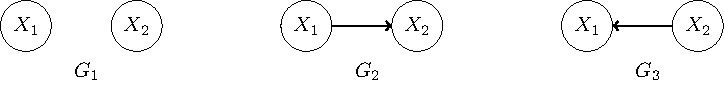
\includegraphics{./picture/bivariate.pdf}
  \caption{2変数のPoisson-DAGモデル}
  \label{fig:ex_bivariate}
\end{figure}

命題\ref{prop:MRS}より、$G_1$におけるすべての頂点$j \in \{ 1,2 \}$について、
$E(X_j^2) = E(X_j) + E(X_j)^2$である。
$G_2$においては、以下が成り立つ。
\begin{equation*}
  E(X_1^2) = E(X_1) + E(X_1)^2, \quad \text{かつ} \quad
  E(X_2^2) > E(X_2) + E(X_2)^2
\end{equation*}
同様に、$G_3$においては、以下が成り立つ。
\begin{equation*}
  E(X_1^2) > E(X_1) + E(X_1)^2, \quad \text{かつ} \quad
  E(X_2^2) = E(X_2) + E(X_2)^2
\end{equation*}
つまり、モーメント比$E(X_j^2) / (E(X_j) + E(X_j)^2)$によって、
真のグラフ構造を同定することが可能である。

命題\ref{prop:MRS}のモーメント比を用いる方法は、
一般的な$p$変数のQVF DAGモデルにも適用することが可能であり、
モーメント比~\eqref{eq:MRS}が1か1以上かを確かめることで識別可能性を証明することができる。

\begin{theo}[QVF DAGモデルの識別可能性]
  2次分散関数性を満たす係数$(\beta_{j0}, \beta_{j1})_{j \in V}$が存在し、
  QVF DAGモデルのクラス\eqref{eq:factorization}について考える。
  任意の頂点$j \in V$について、$\beta_{j1} > -1$であり、
  リンク関数$g_j(\cdot)$が非退化であるならば、
  QVF DAGモデルは識別可能である。
\end{theo}

\begin{proof}
  一般性を失わずに、真の因果順序が一意であり、$\pi = (\pi_1, \dots, \pi_p)$であると仮定する。
  また、簡単のために、$X_{1:j} = (X_{\pi_1}, X_{\pi_2}, \dots, X_{\pi_j})$、
  $X_{1:0} = \emptyset$と定義する。
  加えて、モーメント関連関数$f(\mu) = \beta_0 \mu + (\beta_1 + 1)\mu^2$を定義する。
  ここから数学的帰納法を用いてQVF DAGモデルの識別可能性を証明する。

  \begin{quote}
    \underline{\textbf{Step(1)}} \\
    因果順序が最初である$\pi_1$について、
    命題\ref{prop:MRS}を用いると、
    $E(X_{\pi_1}^2) = E(f(E(X_{\pi_1})))$であるのに対し、
    任意の頂点$j \in V \backslash \{ \pi_1 \}$については、
    $E(X_j ^2) > E(f(E(X_j)))$である。
    よって、因果順序が1番目の要素$\pi_1$を特定することができる。
  \end{quote}

  \begin{quote}
    \underline{\textbf{Step(m-1)}} \\
    因果順序が$(m-1)$番目の要素について、
    因果順序が先の$(m-1)$個の要素とその親が正しく推定されていると仮定する。
    つまり、因果順序が($m-1$)番目の要素については、
    $E(X_{\pi_{m-1}}^2) = E(f(E(X_{\pi_{m-1}} | X_{1:(m-2)})))$が成立していると仮定する。
    一方で、任意の頂点$j \in \{\pi_m, \dots, \pi_p \}$については
    以下が成立していると仮定する。
    \begin{equation*}
      E(X_j^2) > E(f(E(X_j | X_{1:(m-2)})))
    \end{equation*}
  \end{quote}

  \begin{quote}
    \underline{\textbf{Step(m)}} \\
    因果順序が$m$番目の要素とその親について考える。
    帰納法の仮定より、$\pi_m$は、
    $E(X_{\pi_m}^2) = E(f(E(X_{\pi_m} | X_{1:(m-1)})))$である。
    一方で、$j \in \{ \pi_{m+1}, \dots, \pi_p \}$については、
    $E(X_j^2) > E(f(E(X_j | X_{1:(m-1)})))$である。
    よって、因果順序が$m$番目の要素$\pi_m$を特定することができる。

    親変数に関しては、$P(G)$の因数分解\eqref{eq:factorization}による
    以下の条件付き独立関係より導くことができる。
    \begin{align*}
      E(X_{\pi_m}^2) &= E(f(E(X_{\pi_m} | X_{1:(m-1)}))) \\
                     &= E(f(E(X_{\pi_m} | X_{Pa(\pi_m)})))
    \end{align*}
    つまり、上記の関係が成立するような最小の集合を
    $X_{1:(m-1)}$の中から$\pi_m$の親として選択することができる。
  \end{quote}
\qed
\end{proof}

Park and Raskutti(2017)\cite{Park2017-hw}によって証明された
QVF DAGモデルの識別可能条件には、
$Pa(j) \nsubseteq S_j$のとき、すべての$x \in \mathcal X_{S_j}$について、
$\mathrm{Var}(E(X_j | X_{Pa(j)}) | X_{S_j} = x) > 0$という
仮定が含まれていた。
しかし、本論文における識別可能条件にはそのような仮定は含まれていない。
なぜなら、2次分散関数性の定義とイェンセンの不等式を利用することで、
式~\eqref{eq:MRS}や式~\eqref{eq:MRS_2}が成立するためである。
つまり、QVF DAGモデルの従来の識別可能条件\cite{Park2017-hw}を緩和している。
このことによって、Park and Park(2019)\cite{Park2019-qy}の3.2節における議論と同様に
QVF-SEMの学習コストを低下させることが期待される。
ただし、本研究の目的から外れるため、学習コストに関する理論的な証明は行わない。


%
%!TEX root = ../thesis.tex

\section{提案モデル}
\label{part:proposal}

本章では前章で俯瞰した2つのモデル\cite{Shimizu2006-yu}\cite{Park2017-hw}を用いることによって、
連続変数と離散変数が混合したデータにおけるDAGモデルを提案し、
その識別可能性を証明する。
その後、提案モデルを推定する手法について述べる。

%
%!TEX root = ../thesis.tex

\subsection{提案モデル}

提案モデルにおける変数は、離散変数と連続変数に分けられ、
離散変数は0以上の整数を取る確率変数であると仮定する。
そこで提案モデルを以下のように定義する。

\begin{enumerate}
  \item
  $p$個の観測変数$X = \{ X_1, \dots, X_p \}$は
  DAGによって表現されるデータ生成仮定から生成されており、
  各変数の親変数がその変数の直接的な原因である。

  \item
  $p$個の観測変数$X = \{ X_1, \dots, X_p \}$は、
  連続変数($X_j \in \mathbb R$)か離散変数($X_j \in \{0, \mathbb N$\})の
  いずれかに割り当てられる。

  \item
  連続変数に割り当てられた変数$X_j$は、
  その親変数$Pa(j)$と誤差変数$e_j$の線形和である。

  \begin{equation}
    X_j = e_j + \theta_{j} + \sum_{k \in Pa(j)} \theta_{jk}X_j
    \quad \text{with} \quad e_j \sim \text{non-Gaussian}
    \label{eq:lingam_prop}
  \end{equation}

  それぞれの係数$\theta_{jk}$は、変数$X_k$から変数$X_j$への直接的な因果効果の大きさを表す。
  また、誤差変数$e_j$は非ガウス分布に従う確率変数であり、お互いに独立である。

  \item
  離散変数に割り当てられた変数$X_j$は、
  その親変数$Pa(j)$による条件付き確率が、2次分散関数性を満たす。
  つまり、以下を満たすような$\beta_{j0},\beta_{j1} \in \mathbb{R}$が存在する。

  \begin{equation}
    \mathit{Var}(X_j|X_{Pa(j)}) = \beta_{j0} E(X_j | X_{Pa(j)}) + \beta_{j1} E(X_j | X_{Pa(j)})^2
    \label{QVF_prop}
  \end{equation}

  また、各変数の条件付き期待値は、
  その変数の親変数$Pa(j)$と
  任意の単調で微分可能なリンク関数$g_j \colon \mathcal X_{Pa(j)} \rightarrow \mathbb R^+$
  によって以下のように記述される。
  \begin{equation}
    E(X_j | X_{Pa(j)})
    = g_j(X_{Pa(j)})
    = g_j \left(\theta_j + \sum_{k \in Pa(j)} \theta_{jk}X_k \right)
  \end{equation}

  ここで、モデルの解釈性を優先させるため、
  リンク関数$g_i$はパラメータ$\theta$に関して線形な関数であることを仮定しているが、
  以降の識別可能性の議論などではそのような仮定は必要ではない。
\end{enumerate}

%
%!TEX root = ../thesis.tex

\subsection{提案モデルの識別可能性}

本節では、前節で提案したDAGモデルの識別可能性を証明する

\textcolor{red}{もう少しまとまってから書く…}


%
%% Appendix
% \appendix{}
% \include{appendix}
%
%% Back Matter
%\backmatter{}
%
\bibliographystyle{jabbrv}
\bibliography{main_bibliography}
\addcontentsline{toc}{section}{参考文献}
%
%!TEX root = ../thesis.tex
%
\section*{謝辞}
\addcontentsline{toc}{section}{謝辞}
%
本研究活動および論文の執筆にあたり、終始適切な助言を賜り、
丁寧に指導してくださった清水昌平先生に感謝申し上げます。
研究を初めた当初は、統計的因果推論に関する知識は全くない状態でしたが、
外部講師を招いた研究会を開催いただいたり、
ゼミにおける輪読会にて真摯にコメントいただいたりしたことで、
分野の理解を深めることができました。
また、副指導教員を引き受けてくださった伊達平和先生には、
中間報告会などにおいて研究内容の意義に対する貴重な助言をいただきました。
感謝申し上げます。
さらに、日頃のゼミにおいて理論に関して丁寧な指導をしてくださった
青山学院大学経営学部の保科架風先生に感謝申し上げます。

そして、社会人派遣学生として送り出してくださった株式会社マクロミルの皆様に感謝いたします。
特に、「社会人を数年間経験してからいつか大学院に進学したい」という自身の希望を聞き入れ、
派遣を推薦してくださった西部君隆さん、
派遣期間中に様々なご支援をいただいた小笠原道明さん、
論文執筆中の諸業務を調整いただいた丸雄太さんに心から感謝いたします。

最後になりましたが、2年間の学生生活を共に切磋琢磨した
データサイエンス研究科修士課程第1期生の皆様、
清水研究室の研究室の皆様に感謝いたします。


%

\end{document}
